\section{Demonstration}\label{apdx:demo}
This section presents examples drawn from a variety of application scenarios, including the initial four positive cases and the final two negative ones. Each example illustrates our API-GUI operational paradigm, which addresses the diverse challenges and requirements that arise within different applications.

\subsection{Create Monthly Sales Summary Table}
The targeted task to be executed is "Create a table with two headers ('Month' and 'Total') in a new sheet to show the total sales for all months." The actual execution steps can be summarized as follows:
\begin{itemize}
    \item Step1: Switch to `Sheet2`
    \item Step2: Set cell `A1` as "Month"
    \item Step3: Set cell `B1` as "Total"
    \item Step4: Get monthly sales data from `Sheet1`
    \item Step5: Switch to `Sheet1`
    \item Step6: Switch to `Sheet2`
    \item Step7: Set month names in column A
    \item Step8: Set total formula for Jan in `B2`
    \item Step9: Set total formula for Feb in `B3`
    \item Step10: Set total formula for Mar in `B4`
    \item Step11: Set total formula for Apr in `B5`
    \item Step12: Set total formula for May in `B6`
    \item Step13: Set total formula for Jun in `B7`
    \item Step14: Exit after completion
\end{itemize}
As Figure~\ref{figs:demo1-1},\ref{figs:demo1-2} shows, a summary table is created successfully.

\subsection{Convert Uppercase Text to Lowercase in Document}
The targeted task to be executed is "Convert all uppercase text to lowercase in the document for consistent text presentation." The actual execution steps can be summarized as follows:
\begin{itemize}
    \item Step1: Use the text case conversion tool to change all text to lowercase.
    \item Step2: Click the formatting menu.
    \item Step3: Select the specific formatting option.
    \item Step4: Open the relevant submenu.
    \item Step5: Select all text in the document.
    \item Step6: Click the formatting menu again.
    \item Step7: Select the specific formatting option again.
    \item Step8: Open the relevant submenu again to apply the changes.
    \item Step9: Exit after finishing the operation.
\end{itemize}
As Figure~\ref{figs:demo2} shows, all uppercase text has been successfully converted to lowercase, ensuring a uniform and polished document appearance.

\subsection{Generate System Resource Monitoring Report}
The targeted task to be executed is "Use the 'sar' command in the 'sysstat' toolkit to monitor system activity and output the results to 'System\_Resources\_Report.txt' under Desktop." The actual execution steps can be summarized as follows:
\begin{itemize}
    \item Step1: Open the Terminal application.
    \item Step2: Type the command \texttt{sar 1 30 >~/Desktop/System\_Resources\_Report.txt}.
    \item Step3: Execute \texttt{sudo apt install sysstat} to install the toolkit.
    \item Step4: Enter the password if prompted.
    \item Step5: Re-type the sar command to start monitoring.
    \item Step6: Wait for 30 seconds while system activity is being recorded.
    \item Step7: Open the Files application.
    \item Step8: Navigate to and click on the report file under Desktop.
    \item Step9: Exit after confirming the report has been generated.
\end{itemize}
As Figure~\ref{figs:demo3} shows, a system resource report file was generated successfully on the Desktop after monitoring, fulfilling the target task.

\subsection{Copy Image from .xcf File to LibreOffice Writer and Save}
The targeted task to be executed is "Copy the image from an \texttt{.xcf} file located on the Desktop and paste it into a LibreOffice Writer document, then save the document as \texttt{image.docx} on the Desktop." The actual execution steps can be summarized as follows:
\begin{itemize}
    \item Step1: Open the Files application.
    \item Step2: Navigate to the Desktop folder.
    \item Step3: Double-click to open the \texttt{.xcf} image file.
    \item Step4: Copy the image in the image editor.
    \item Step5: Open LibreOffice Writer.
    \item Step6: Paste the copied image into the Writer document.
    \item Step7: Save the document.
    \item Step8: Enter the filename as \texttt{image.docx} and select the Desktop as the save location.
    \item Step9: Navigate to the Desktop folder.
    \item Step10: Confirm and click save.
\end{itemize}
As Figure~\ref{figs:demo4-1} shows, the image from the \texttt{.xcf} file was successfully pasted into a LibreOffice Writer document and saved as \texttt{image.docx} on the Desktop, completing the task.

\subsection{Question Misunderstanding Error}
The targeted task to be executed is "Append \texttt{<br/>} to the end of each line in '1\textbackslash n2\textbackslash n3' and save in output.txt." The actual execution steps can be summarized as follows:
\begin{itemize}
    \item Step1: Type the command \texttt{echo -e '1\textbackslash n2\textbackslash n3'} in the terminal.
    \item Step2: Exit after execution.
\end{itemize}
As Figure~\ref{figs:bad1} shows, the agent misunderstood the requirement and only echoed the content without appending \texttt{<br/>} to each line or saving it into output.txt. This results in a task failure due to a misunderstanding of the question.

\subsection{Click Operation Error}
The targeted task to be executed is "Please help change GIMP's theme from dark to light." The actual execution steps can be summarized as follows:
\begin{itemize}
    \item Step1: Click on the menu in GIMP.
    \item Step2: Attempt to click the Preferences option.
    \item Step3: Repeat the click on Preferences.
    \item Step4: Try to use the shortcut \texttt{Shift+Ctrl+P} to open Preferences.
    \item Step5: Exit without successfully changing the theme.
\end{itemize}
As Figure~\ref{figs:bad2} shows, the theme remains dark, indicating that the agent failed to change GIMP's theme to light due to incorrect click operations.

\begin{figure}[t]
    \centering
    \includegraphics[width=0.95\textwidth]{images/demo1-1.pdf}
    \vspace{-2mm}
    \caption{Task (Step 1-10): Create a table with two headers ("Month" and "Total") in a new sheet to show the total sales for all months.}
    \label{figs:demo1-1}
\end{figure}

\begin{figure}[t]
    \centering
    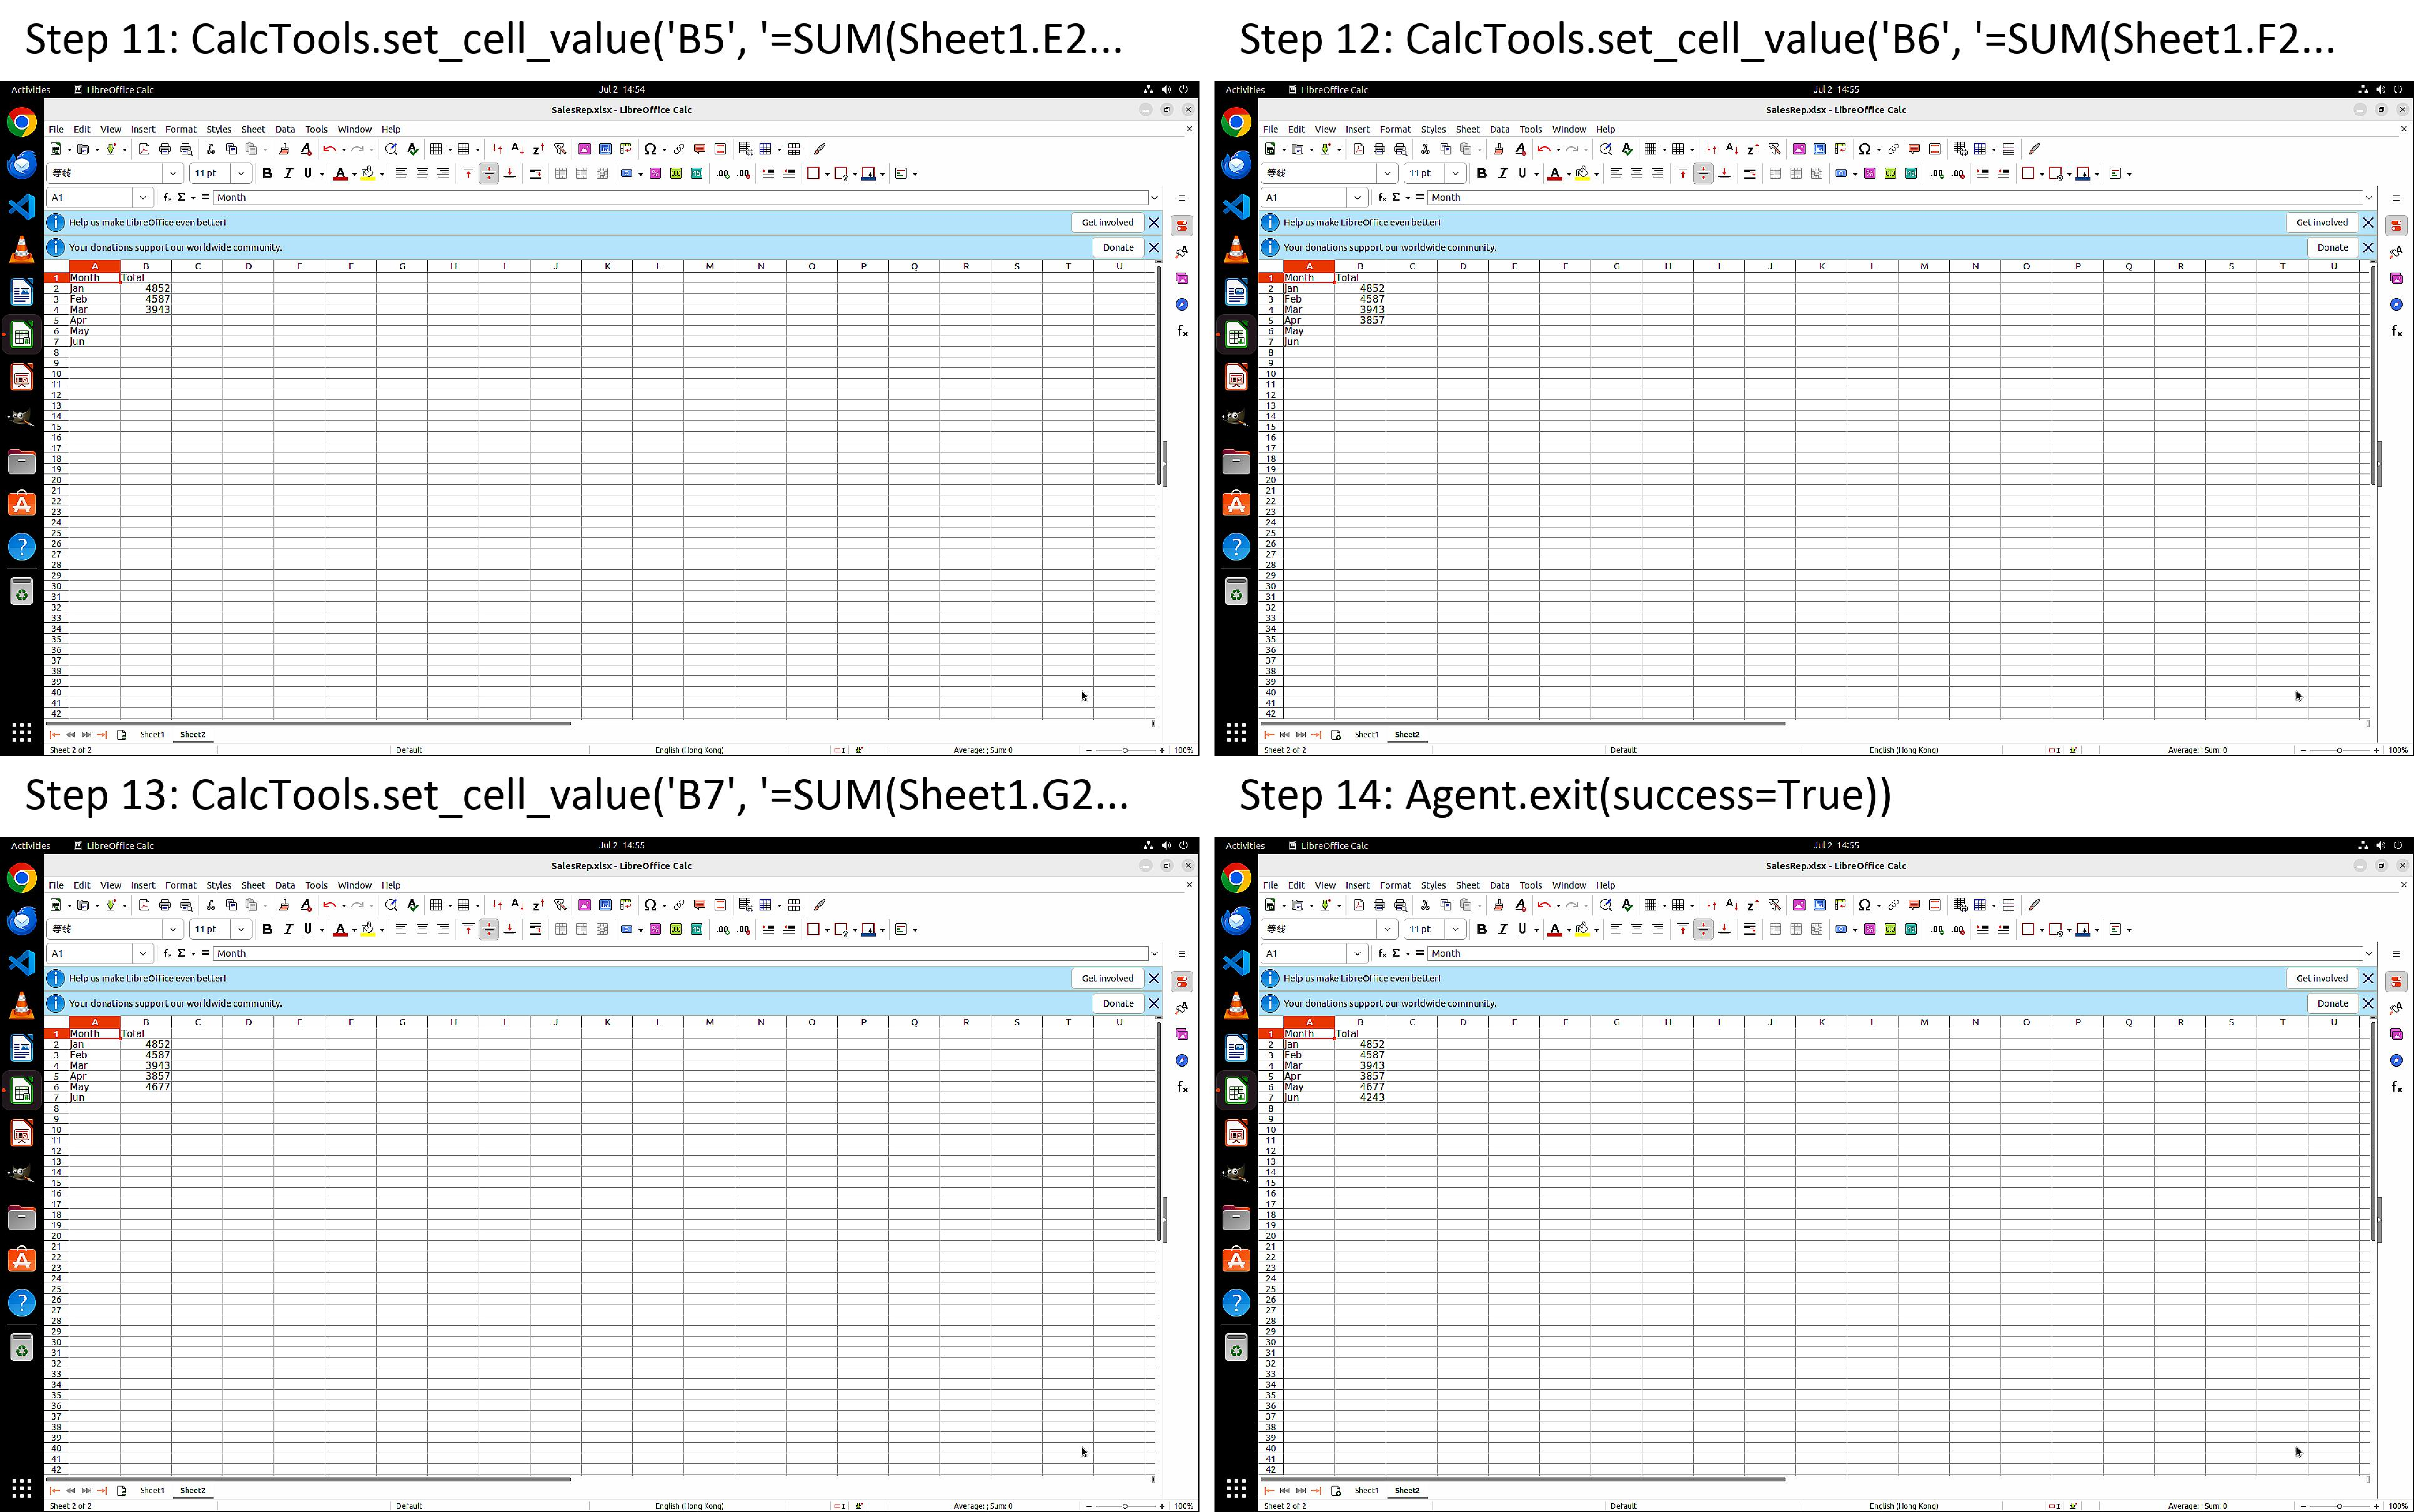
\includegraphics[width=0.95\textwidth]{images/demo1-2.pdf}
    \vspace{-2mm}
    \caption{Task (Step 11-14): Create a table with two headers ("Month" and "Total") in a new sheet to show the total sales for all months.}
    \label{figs:demo1-2}
\end{figure}

\begin{figure}[t]
    \centering
    \includegraphics[width=0.95\textwidth]{images/demo2.pdf}
    \vspace{-2mm}
    \caption{Task: I am currently engaged in text processing and require assistance in converting all uppercase text to lowercase within my document. This precision is critical for maintaining a uniform and polished presentation. Could you help me on this?}
    \label{figs:demo2}
\end{figure}

\begin{figure}[t]
    \centering
    \includegraphics[width=0.95\textwidth]{images/demo3.pdf}
    \vspace{-2mm}
    \caption{Task: Please use the `sar` command in the `sysstat` toolkit to monitor system activity, evaluate the status once every second for 30 seconds, output the results to "System\_Resources\_Report.txt" under Desktop.}
    \label{figs:demo3}
\end{figure}

\begin{figure}[t]
    \centering
    \includegraphics[width=0.95\textwidth]{images/demo4-1.pdf}\
    \vspace{-2mm}
    \caption{Task: I've stored my .xcf file on the Desktop. Can you assist me in copying the image and pasting it into a LibreOffice Writer document? Save the document as 'image.docx' on the Desktop, please.}
    \label{figs:demo4-1}
\end{figure}

% \begin{figure}[t]
%     \centering
%     \includegraphics[width=1.0\textwidth]{images/demo4-2.pdf}
%     \caption{demo4-2}
%     \label{figs:demo4-2}
% \end{figure}

\begin{figure}[t]
    \centering
    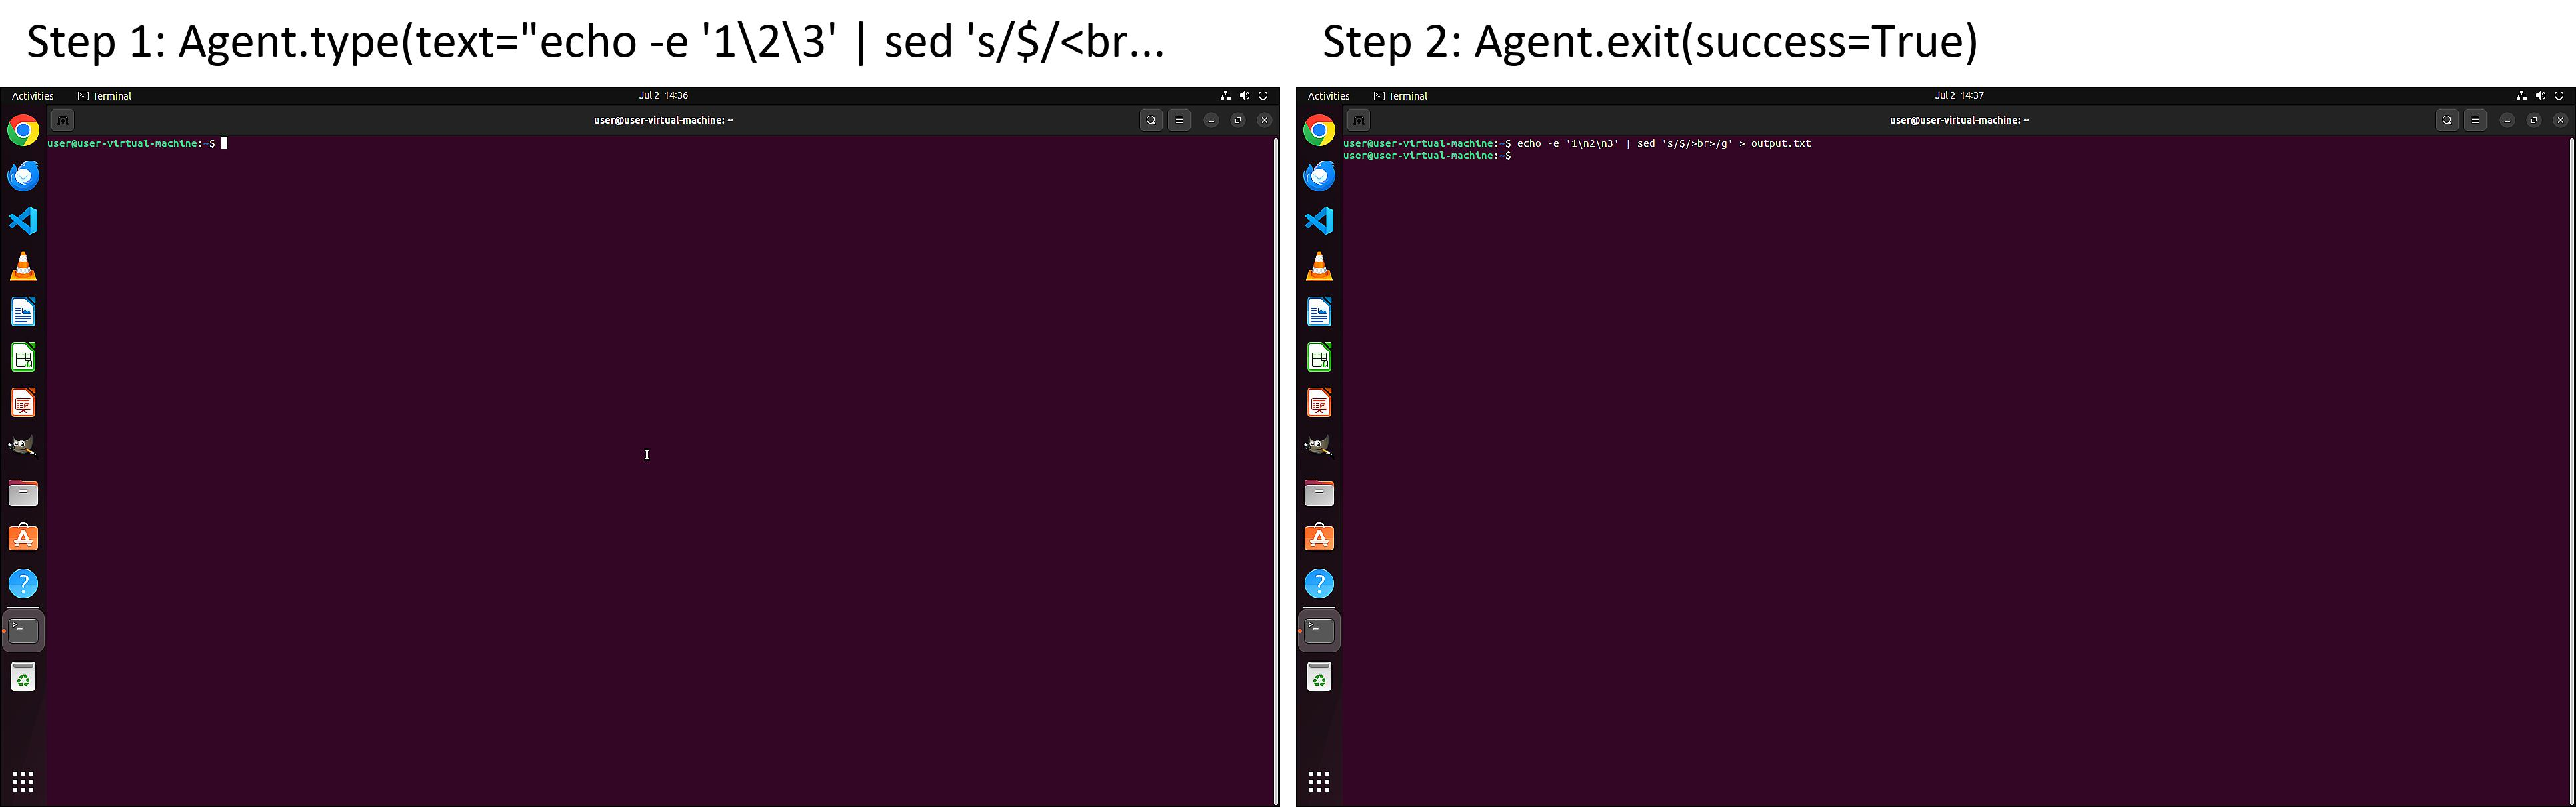
\includegraphics[width=0.95\textwidth]{images/bad-1.pdf}
    \vspace{-2mm}
    \caption{Fail Task (Question Misunderstanding Error): Append "<br/>" to the end of each line in "1\textbackslash n2\textbackslash n3" and save in output.txt}
    \label{figs:bad1}
\end{figure}

\begin{figure}[t]
    \centering
    \includegraphics[width=0.95\textwidth]{images/bad-2.pdf}
    \vspace{-2mm}
    \caption{Fail Task (Click Operation Error): Please help change GIMP's theme from dark to light.}
    \label{figs:bad2}
\end{figure}